\chapter{Interferometric sensitivity to the global signal}
\label{chapter:TAV}

As described in Chapter~\ref{chapter:eor_intro}, the EoR global signal contains key information about the thermal history of the IGM as a function of redshift, across $80<z<6$ at the least. Observational efforts to detect the global signal typically consist of a single element (or duplicates of a single element for systematic cross-checks), while interferometric measurements concentrate on the anisotropic signal. 

Traditionally, an interferometer is not regarded as sensitive to the average signal on the sky. Indeed, in the limit of a flat, infinite sky, the sky-averaged visibility of any pair of baselines is identically zero. This is because the average signal is equivalent to the ($u,v$) = (0,0) spatial Fourier mode, which for interferometers with narrow fields-of-view is inaccessible as the two antennae would need to be co-incident.
However, when the flat-sky approximation is no longer valid, a monopole moment may be detectable in principle. \cite{Presley.15} argued that the curved nature of the sky implies the integrated response of an interferometer to a constant signal is not zero. Experimentally, these types of results are quite exciting, because the full power of cross-correlation -- negation of correlated noise and increased sampling of Fourier modes -- can be brought to bear on the problem of very bright foregrounds. As a result, it may be possible to detect the 21\,cm global signal without the necessity of performing extensive self-calibration of an individual antenna response.

However, \cite{Venumadhav.16} presented a general argument that an interferometer is not sensitive to the global signal, except by means of instrument imperfections. They argued that sensitivity to a global signal only enters an interferometric measurement by way of: (1) direct cross-talk between two antennas, (2) cross-talk between two antennas by way of a mutual coupling with a third antenna, or (3) a mutual coherent noise source between two antennas. The authors claimed that upon performing a cross-correlation operation on the received voltage measurements, any correlations disappear. They also claimed that interferometers are incapable of understanding these noise properties.

In this Chapter, we present a formalism that shows that interferometers may be sensitive to the global signal. Our analysis is complimentary to the one presented by \cite{Presley.15}, but approaches the problem from a more spherical basis. We also present measurements that are suggestive, but not conclusive, of measurements of the global signal of Galactic foregrounds with the PAPER interferometer. We assume the Condon-Shortley phase convention throughout \citep{Condon.51}.

\section{Mathematical Formalism}
\label{sec:global_signal_math}
We wish to answer the question of whether an interferometer can measure the
spherical harmonic monopole, that is, the specific mode $\ell = m =
0$. The main characteristic of this mode is constant power, coming from all angles
$\Omega$ on the sky. We assume, however, that this emission from any particular
pointing $\hat{s}$ is \textit{incoherent} with that from any other direction,
but that the average emission in any direction is the same. 

In other words, we
assume that the emitters in the far field of the instrument are uncorrelated,
and thus the monopole moment of the radiation satisfies
\begin{equation}
\frac{1}{Z_0} \left\langle \vec{E}(\hat{r})\vec{E}(\hat{r}') \right\rangle = P(\nu) \delta(\hat{r} - \hat{r}').
\end{equation}
The power received in independent of direction, but the fields in any two
directions are uncorrelated.

To gain insight into how an interferometer responds to an isotropic sky
signal, we will begin with the classical interferometric visibility equation. We note that
there are several assumptions that enter to the visibility equation, though
these are typically well-justified in the applications of interest. In
particular, we assume that:
\begin{enumerate}
\item The emission is in the far field of the pair of antennas.
\item The emission is incoherent.
\item The antennas do not affect one another's radiation patterns.
\item The antennas or their structures do not scatter the incident radiation.
\item The antennas are perfectly terminated and do not reflect incident radiation.
\item There is no loss in the antennas elements except for at the detector.
\end{enumerate}
In general, all of these assumptions except for (1) and (2) are violated for
real experiments. As noted in \cite{Venumadhav.16}, an important
consideration for an interferometer's sensitivity to the monopole is the
sensitivity along the line of sight connecting the two antennas. Thus, the
extent to which assumptions (3--5) hold will affect the extent to which an
interferometer is theoretically sensitive to the sky monopole.

\subsection{Spherical Harmonic Transform of the Visibility Equation}

We can rewrite the visibility observed by baseline $\vec{b}$ (with horizon-delay of $\tau_h = b/c$) by expanding the fringe term using spherical harmonics and spherical Bessel functions:
\begin{equation}
\exp\left(-2\pi i \nu \tau_h \hat{b}\cdot\hat{s}\right) = 2\pi \sum_{\ell, m} (-i)^{\ell} j_{\ell}(2\pi\tau_h\nu) Y^m_{\ell}(\hat{b}) Y^{m*}_{\ell}(\hat{s}),
\label{eq:tav_fringe_expansion}
\end{equation}
and expanding the chromatic beam ($A(\hat{s},\nu)$) and sky terms ($S(\hat{s},\nu)$) in terms of spherical harmonics:
\begin{equation}
A(\hat{s},\nu) = \sum_{\ell, m} a_{\ell, m}(\nu)Y^m_{\ell}(\hat{s}),
\end{equation} 
\begin{equation}
S(\hat{s},\nu) = \sum_{\ell, m} s_{\ell, m}(\nu)Y^m_{\ell}(\hat{s}).
\end{equation} 
Finally, we can write Equation~\ref{eq:tav_fringe_expansion} consistently with the above two terms:
\begin{equation}
\exp\left(-2\pi i \nu \tau_h \hat{b}\cdot\hat{s}\right) = \sum_{\ell, m} f_{\ell, m}(\hat{b},\nu) Y^{m*}_{\ell}(\hat{s}),
\end{equation}
where we have defined a `fringe harmonic' term:
\begin{equation}
f_{\ell, m}(\hat{b},\nu) \equiv 2\pi \sum_{\ell, m} (-i)^{\ell} j_{\ell}(2\pi\tau_h\nu) Y^m_{\ell}(\hat{b}).
\end{equation}
Combining all of the above allows us to formulate the classical visibility equation as a sum of spherical harmonic terms, which we will denote using separate indices:
\begin{equation}
V(\nu) = \sum_{\substack{\ell_1, m_1 \\ \ell_2, m_2 \\ \ell_3, m_3}} a_{\ell_1, m_1} (\nu) s_{\ell_2, m_2} (\nu) f_{\ell_3, m_3} (\hat{b}, \nu) \times \int Y_{\ell_1}^{m_1} (\hat{s}) Y_{\ell_2}^{m_2} (\hat{s}) {Y_{\ell_3}^{m_3}}^* (\hat{s}) {\rm d}\Omega.
\label{eq:vgeneral}
\end{equation}
The integral over $\Omega$ can be expressed in terms of  Wigner-$3j$ symbols \citep{Wigner.51}:
\begin{multline}
\int Y_{\ell_1}^{m_1} (\hat{s}) Y_{\ell_2}^{m_2} (\hat{s}) {Y_{\ell_3}^{m_3}}^* (\hat{s}) {\rm d}{\hat{s}} = \\
\sqrt{\frac{(2\ell_1 + 1)(2\ell_2 + 1)(2\ell_3 + 1)}{4\pi}} \\
\times \begin{pmatrix}
\ell_1 & \ell_2 & \ell_3 \\
0 & 0 & 0
\end{pmatrix}
\begin{pmatrix}
\ell_1 & \ell_2 & \ell_3 \\
m_1 & m_2 & -m_3
\end{pmatrix}
\end{multline}

\subsection{Coupling to the Sky Monopole}
Thus far, we have made no assumptions about the form of the terms in the visibility equation. The sky monopole is defined in our notation as $\ell_2 = m_2 = 0$. For these modes, the Wigner-$3j$ symbols can undergo two odd permutations of the columns:
\begin{equation}
\begin{pmatrix}
\ell_1 & 0 & \ell_3 \\
0 & 0 & 0
\end{pmatrix}
\begin{pmatrix}
\ell_1 & 0 & \ell_3 \\
m_1 & 0 & -m_3
\end{pmatrix}
=
\begin{pmatrix}
\ell_1 & \ell_3 & 0 \\
0 & 0 & 0
\end{pmatrix}
\begin{pmatrix}
\ell_1 & \ell_3 & 0 \\
m_1 & -m_3 & 0
\end{pmatrix}
\end{equation}
which will have the resultant selection rules:
\begin{equation}
| \ell_1 - \ell_3 | \leq 0 \leq \ell_1 + \ell_3;\,\,\,m_1 - m_3 = 0.
\end{equation}
These constraints require that $\ell_1 = \ell_3 \equiv \ell$ and $m_1 = m_3 \equiv m$, resulting in the factor
\begin{equation}
\begin{pmatrix}
\ell & \ell & 0 \\
0 & 0 & 0
\end{pmatrix}
\begin{pmatrix}
\ell & \ell & 0 \\
m & -m & 0
\end{pmatrix}
= \frac{(-1)^m}{2\ell + 1}.
\end{equation}

We can define a component of the visibility containing the sky monopole $s_{00}$ as 

\begin{equation}
V_0(\nu) = \frac{s_{00}(\nu)}{\sqrt{4\pi}} \sum_{\ell, m} (-1)^m a_{\ell, m}(\nu) f_{\ell,m}(\hat{b},\nu) = s_{00}(\nu)\Xi(\hat{b},\nu)
\label{eq:xi_def}
\end{equation}
where $\Xi(\hat{b},\nu)$ is a transfer function containing the response of the beam and fringe terms to the monopole. If $\Xi(\hat{b},\nu)$ is non-zero, the interferometer is capable of measuring the global signal.

\section{Analytic and Numeric Calculations}

The expression for $\Xi(\hat{b},\nu)$ shows that the sensitivity to the monopole is closely connected to the baseline length and spherical harmonic coefficients of the beam. One can expand a given model beam and baseline to an arbitrary $\ell, m$. The spherical Bessel function falls exponentially with $\ell$, so the sum should converge.

\subsection{Toy Model}
\label{subsec:toy_model}
To build intuition, we implement a simple toy model for $V_0(\nu)$. We assume a global sky model of $s_{00}(\nu) = S_0\nu^{-\alpha}$ (which is roughly consistent with current global low-frequency measurements \citealt{Mozden.17}), and a beam model such that $a_{00}(\nu) = A_0\nu^{-\beta}$. We only endeavour to calculate the ($\ell,m$) = (0,0) component; the first term of the sum. Figure~\ref{fig:xi_toy} shows $\Xi(\hat{b},\nu)$ for $\alpha=1.5$, $\beta = 1$. 

\begin{figure}
\centering
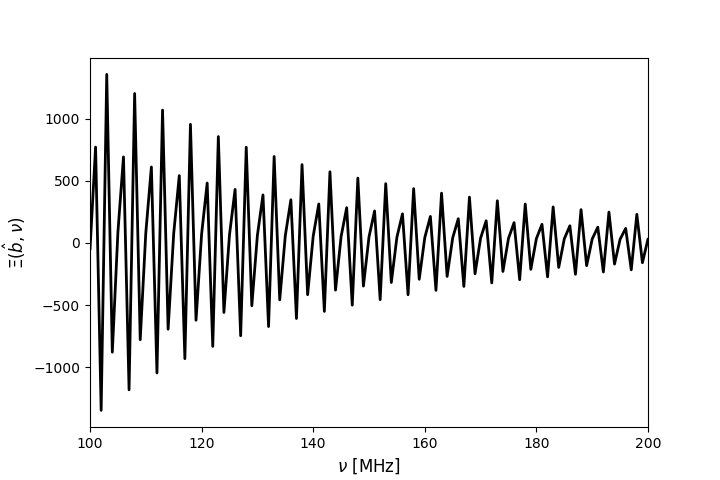
\includegraphics[width=0.8\textwidth]{chapters/global_signal/figures/xi_toy.png}
\caption[The transfer function for a simple beam and sky model.]{The transfer function for a simple beam and sky model, both as power laws in harmonic space, and only using the ($\ell,m$) = (0,0) mode, for a 30\,m East-West baseline.}
\label{fig:xi_toy}
\end{figure}

As we will find below, using the delay transform \citep{Parsons.12b} is an extremely useful method for understanding whether or not fringing, multipolar terms are present in the data. For this toy model, the delay transform $\tilde{V}_{00}(\tau)$ can be expressed analytically:

\begin{multline}
\tilde{V}_{00}(\tau) = i^{1 + 3(\alpha+\beta)} \frac{s_0 a_0 (2\pi)^{\alpha+\beta}}{4\pi\tau_h} \\
\times \Big[(\tau-\tau_h)^{\alpha+\beta}\Gamma_{+--} - (\tau-\tau_h)^{\alpha+\beta}\Gamma_{-+-} \\
 - (\tau+\tau_h)^{\alpha+\beta}\Gamma_{+-+} + (\tau+\tau_h)^{\alpha+\beta}\Gamma_{-++}\Big], 
\label{eq:vg}
\end{multline}
where the functions $\Gamma_{\pm\pm\pm}$ are defined as
\begin{equation}
\Gamma_{\pm\pm\pm} \equiv \Gamma(-\alpha-\beta, \pm i \pi (B \pm 2\nu_0)(\tau \pm \tau_h)),
\end{equation}
and $\Gamma(s, z)$ is the upper incomplete Gamma function.

In Figure~\ref{fig:vg_tau}, we show the delay transform for $\alpha=1.5$ and $\beta=0$ (i.e. no frequency evolution) and $\beta=1$ for a 30\,m baseline. Clear in both Equation~\ref{eq:vg} and Figure~\ref{fig:vg_tau} is the selection of the horizon delay (100\,ns) as the location of monopole signal in delay space. 
The interpretation of this effect is that while the monopole, by definition, emits across the sky, an interferometer is maximally sensitive to it at the horizon. This is the location where the baseline vector is coincident with the $\hat{s}$ term integrated-over in the visibility equation. \cite{Venumadhav.16} showed the same effect (see their Section 5), but not in the delay formalism.

\begin{figure}
\centering
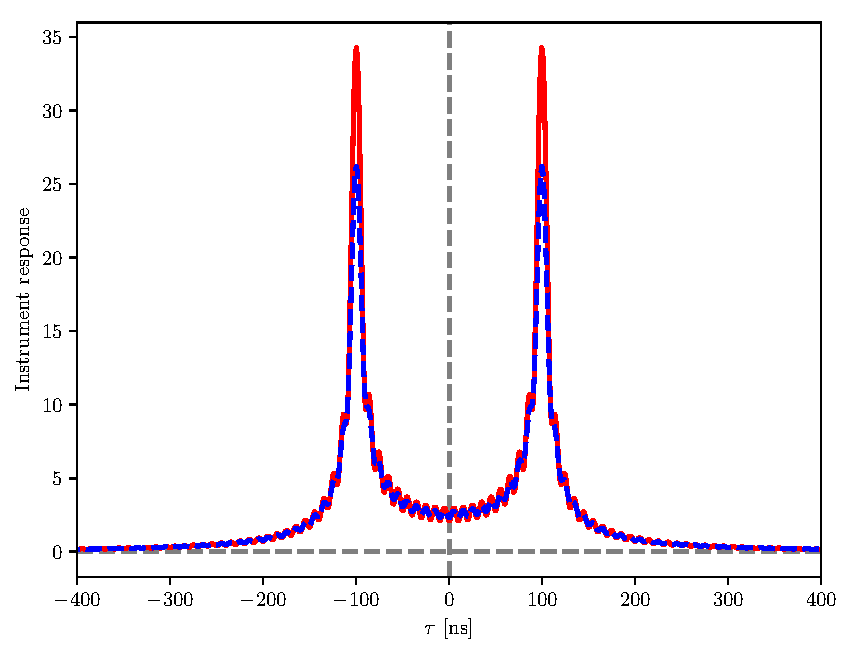
\includegraphics[width=0.8\textwidth]{chapters/global_signal/figures/vg.pdf}
\caption[The delay transform of the interferometer response to the monopole
    moment of the global signal, including only the zeroth-order response of the
    instrument.]{The delay transform of the interferometer response to the monopole
    moment of the global signal, including only the zeroth-order response of the
    instrument. The functional form of this result is given by
    Equation~\ref{eq:vg}. The plot uses a value of $\alpha = 1.5$ for the
    power law index of the monopole moment, and $\beta = 0$ (solid red curve)
    and $\beta = 1$ (dashed blue curve) as the power law index for the
    instrument response. The light-crossing time separation between the antennas
    $\tau_h$ was chosen to be 100 ns, which sets the location of the peaks in
    the delay spectrum. As can be seen, the chromaticity of the beam smooths out
    the curve somewhat. The $y$-axis has arbitrary units.}
\label{fig:vg_tau}
\end{figure}

The prefactor of Equation~\ref{eq:vg} also indicates that the power in delay space will decrease with baselines of increasing length. This is illustrated in Figure~\ref{fig:vg_tau_three}, which shows $\tilde{V}_{00}(\tau)$ for three baselines of increasing length. The largest response for each of the lengths occurs at the value of $\tau\approx\tau_h$, and the amplitude decreases accordingly. Note that the strength and location in delay space are exactly in in line with the simulations of \cite[][see their Figure 2]{Nithya.15b}, although the main purpose of their study was simulating the power spectrum response of different interferometers. This relationship was also predicted by \cite{Venumadhav.16}.

\begin{figure}
\centering
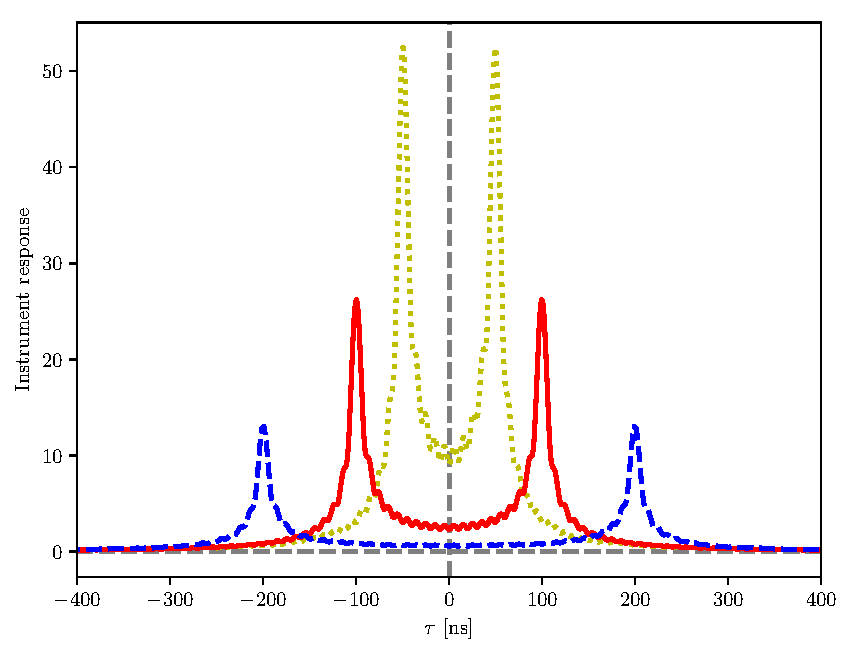
\includegraphics[width=0.8\textwidth]{chapters/global_signal/figures/vg_th.pdf}
\caption[The delay transform for different values of $\tau_h$.]{
    The delay transform for different values of $\tau_h$ for a fixed
    value of $\beta = 1$. The values of $\tau_h$ are $\tau_h = 50$ ns (dotted
    yellow line), $\tau_h = 100$ ns (solid red line), and $\tau_h = 200$ ns
    (dashed blue line). Note that in all cases, the largest response occurs when
    $\tau \approx \tau_h$. Further, note that the amplitude of the response is
    inversely proportional to the value of $\tau_h$: smaller values of $\tau_h$
    result in a larger response.}
\label{fig:vg_tau_three}
\end{figure}

\subsection{Instrument Simulation}
Using the Jones formalism developed in Chapter~\ref{chapter:interferometry} (also see Chapter~\ref{chapter:eor_window_HERA}) and a complex-voltage model of the PAPER \citep[e.g.][]{Parsons.10} dipole beam \citep{Pober.12}, we were able to simulate $\Xi(\hat{b},\nu)$. Figure~\ref{fig:paper_jones} shows the direction-dependent Mueller matrix for the PAPER beam at 150\,MHz. Note the separate color maps for $I\rightarrow I$, the other diagonal terms, and the off-diagonal ones, which we use for dynamic range changes in order capture sufficient detail. The dipole beam, as expected, extends across the sky.

\begin{figure}
\centering
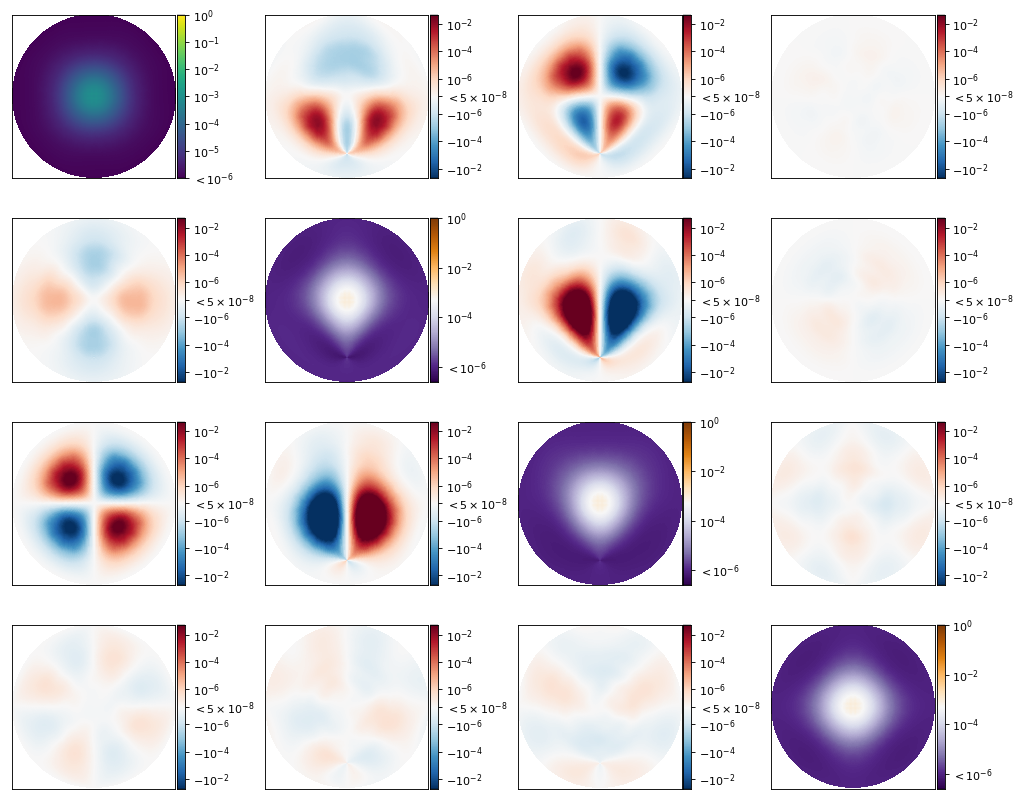
\includegraphics[width=0.8\textwidth]{chapters/global_signal/figures/full_mueller_150MHz.png}
\caption[The direction-dependent Jones matrix for a model PAPER beam at 150 MHz.]{The direction-dependent Jones matrix for a model PAPER beam at 150 MHz. For a review of Jones matrices, see Chapter~\ref{chapter:interferometry}. Note the separate color maps for $I\rightarrow I$, the other diagonal terms, and the off-diagonal ones, which we use for dynamic range changes in order capture sufficient detail.}
\label{fig:paper_jones}
\end{figure}

Figure~\ref{fig:xi_vis} shows the value of $\Xi(\hat{b},\nu)$ as a function of frequency computed from the beam models from Figure~\ref{fig:paper_jones}, for East-West (`ee') and North-South (`nn') instrumental linear polarizations. The non-zero nature of the curves represent that the global signal is, in principle, measurable from interferometric visibilities. However, as shown in Equation~\ref{eq:xi_def}, in order to measure the global signal $s_{00}(\nu)$, $\Xi(\hat{b},\nu)$ must be fit-out from the visibility $V_0(\nu)$ (the fact that the visibility shown in Equation~\ref{eq:xi_def} contains only the monopole sky will be discussed below). 
%Given the oscillatory structure calculated, avoiding null division will require extremely precise modelling as a function of frequency, coupled with extremely accurate phase calibration of the visibility.

\begin{figure}
\centering
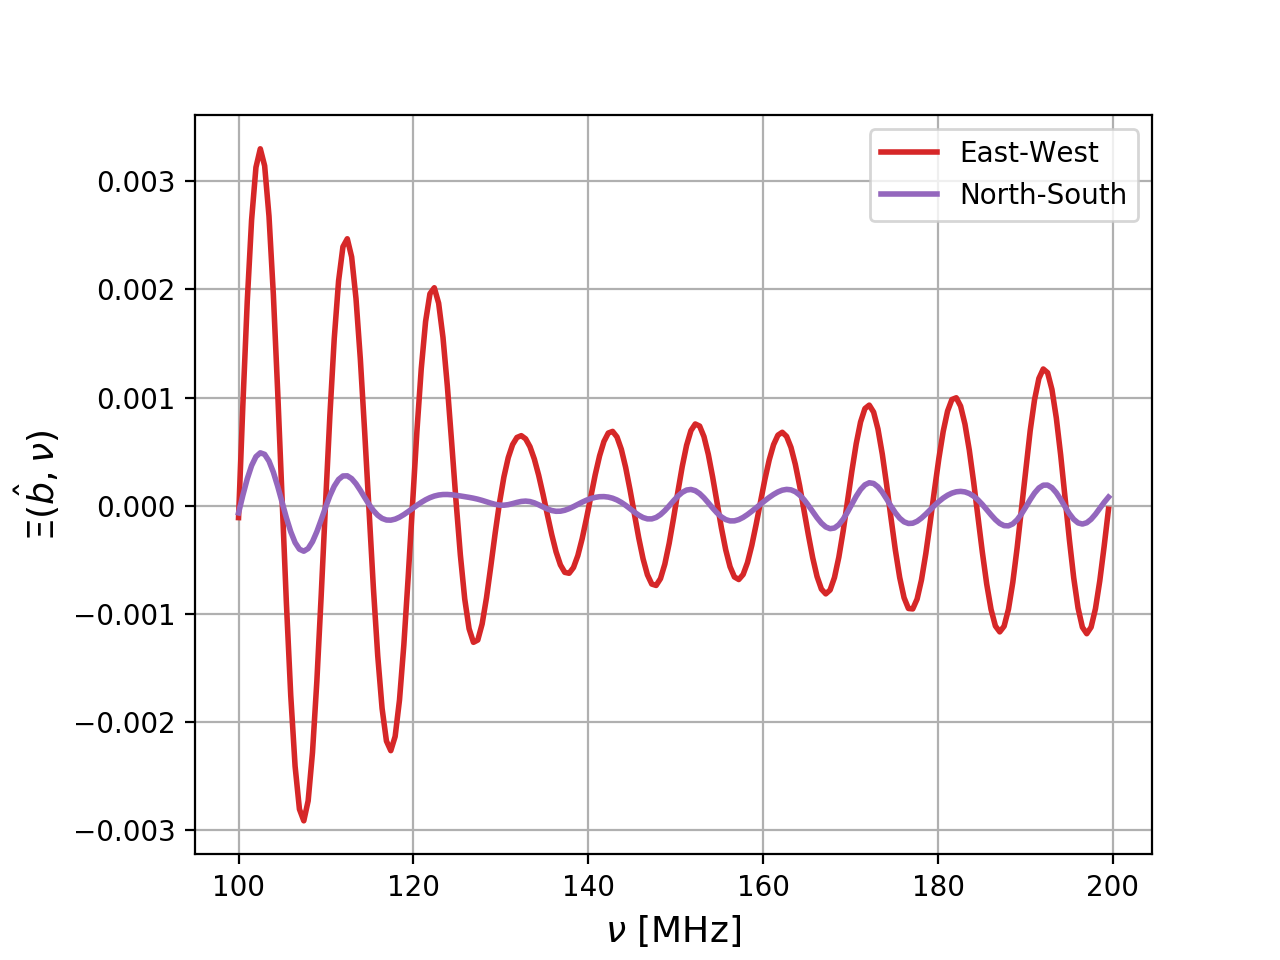
\includegraphics[width=0.8\textwidth]{chapters/global_signal/figures/Xi_vis.png}
\caption[The global signal transfer function as a function of frequency for PAPER.]{The global signal transfer function as a function of frequency for PAPER. It's non-zero nature indicates that the global signal is in principle measurable by an interferometer. However, as $\Xi(\hat{b},\nu)$ must be divided-out of the visibility, the many nulls represent a stringent calibration challenge.}
\label{fig:xi_vis}
\end{figure}

\subsection{Attenuating other harmonics}

Of course, the visibility $V_0(\nu) = s_{00}(\nu)\Xi(\hat{b},\nu)$ contains only the monopole signal of the sky to begin with. The visibility equation is linear, so the total visibility observed can be represented as $V(\nu) = V_0(\nu) + V_{>0}(\nu)$. There are several ways one could separate $V_{>0}(\nu)$ from the total visibility, but for drift-scanning telescopes with long observing seasons, the simplest solution is just to average visibilities over time. 

The expression in Equation~\ref{eq:vgeneral} does not take time into account -- it is the instantaneous visibility. For a drift-scanning interferometer, time dependence is only introduced by the rotation of the Earth. In the formalism above, this can be introduced by multiplication of a factor $\exp\left(-i m_2 \omega_{\Earth} t\right)$, where $m_2$ is an index of the spherical harmonic modes of the sky and $\omega_{\Earth}$ is the rate of the Earth's rotation. The symmetry of $m$-modes with respect to $\ell$ cause an sum over these terms to select the $m_2=0$ mode. In the resultant expression:

\begin{multline}
\left\langle V(\nu, t) \right\rangle_t = 
\sum_{\substack{\ell_1, m_1 \\ \ell_2 \\ \ell_3, m_3}} a_{\ell_1, m_1} (\nu) s_{\ell_2, 0} (\nu) f_{\ell_3, m_3} (\hat{b}, \nu) \times \\
\sqrt{\frac{(2\ell_1 + 1)(2\ell_2 + 1)(2\ell_3 + 1)}{4\pi}}
\times \begin{pmatrix}
\ell_1 & \ell_2 & \ell_3 \\
0 & 0 & 0
\end{pmatrix}
\begin{pmatrix}
\ell_1 & \ell_2 & \ell_3 \\
m_1 & 0 & -m_3
\end{pmatrix},
\end{multline}
the second Wigner-3$j$ symbol obeys the selection rule that $m_1 = m_3$. 
Performing one odd permutation of this second Wigner-3$j$ symbol, and expressing both Wigner-3$j$ symbols as Clebsch-Gordan coefficients:
\begin{equation}
\begin{pmatrix}
\ell_1 & \ell_2 & \ell_3 \\
0 & 0 & 0
\end{pmatrix}
\begin{pmatrix}
\ell_1 & \ell_2 & \ell_3 \\
m_1 & 0 & -m_3
\end{pmatrix}
\propto
\left\langle \ell_1 0 \ell_2 0 | \ell_3 0 \right\rangle \left\langle \ell_1 m \ell_3 -m | \ell_2 0 \right\rangle,
\end{equation}
it can be shown (e.g. Varshalovich, Moskalev \& Khersonskii, 1988) that the second coefficient obeys the selection rule that $\ell_2 = m_2 = 0$. This shows that time-averaging selects the monopole term of the sky. However, all of the selection rules above stemmed from a totally symmetric averaging of the spherical harmonic modes of the sky. To ensure this is the case, long time-averages are required.

\section{Time-averages from PAPER}

The Season 1 Epoch 2 observations of PAPER-128 were defined and described in Chapter~\ref{chapter:eor_window_psa128}. In Chapters~\ref{chapter:instruments}, \ref{chapter:data_prep_and_proc} and \ref{chapter:eor_window_psa128} we elaborated upon the instrumental design, quality assurance metrics and compression implemented on the data. Season 1 Epoch 2 consists of $\sim 45$ nights of well-characterized observations. In this Chapter, we used Season 1 Epoch 2 PAPER-128 data that was quality assured, and calibrated using the {\sc omnical} \citep{Zheng.14} \textit{4pol+minV} calibration scheme (see Chapter~\ref{chapter:polcal}). 

We then extracted only the 30\,m East-West baselines, in the instrumental `nn' polarization, for analysis. Unlike in Chapter~\ref{chapter:eor_window_psa128}, we did not implement a foreground avoidance scheme. The data were gridded and binned according to their LST of observation, and absolute-calibrated according to the flux density and position of Pictor A at transit \citep[][the same calibration shown in Chapter~\ref{chapter:eor_window_psa128}]{Jacobs.13}.

To isolate the global component of the signal, which does not `fringe' on the sky as observed by the interferometer, we averaged all LSTs into a single frequency spectrum. The real part of the averaged spectrum is shown in the upper panel of Figure~\ref{fig:global_signal_data_vs_sim}, with the simulated PAPER transfer function (Figure~\ref{fig:xi_vis}) over-plotted for reference. The delay transforms of the two spectra are shown in the lower panel of the Figure.

There were some enticing qualitative agreements. Clearly, the phases of the oscillations between simulation and data were very similar to one another; noticeable in the upper panel and very clear in the lower one. 
The power within the foreground wedge region (e.g. Chapter~\ref{chapter:eor_window_theory}) was at the level of noise in the EoR window, indicating that foregrounds were attenuated at the appropriate delays, save, of course, the horizon delays.

As predicted by the toy model in Section~\ref{subsec:toy_model}, the only unattenuated foreground signal appeared at the horizon delays of the 30\,m East-West baselines used in this analysis. As noted above, the observed and simulated delays aligned almost perfectly in delay space. This indicated that the dipole beam, as expected, was accurately described by a small number of spherical harmonic modes. The width of the peaks is determined by the width of the beam in delay space: that the simulated and observed widths matched relatively closely was indicative of an accurate polarized beam model. 

\begin{figure}
\centering
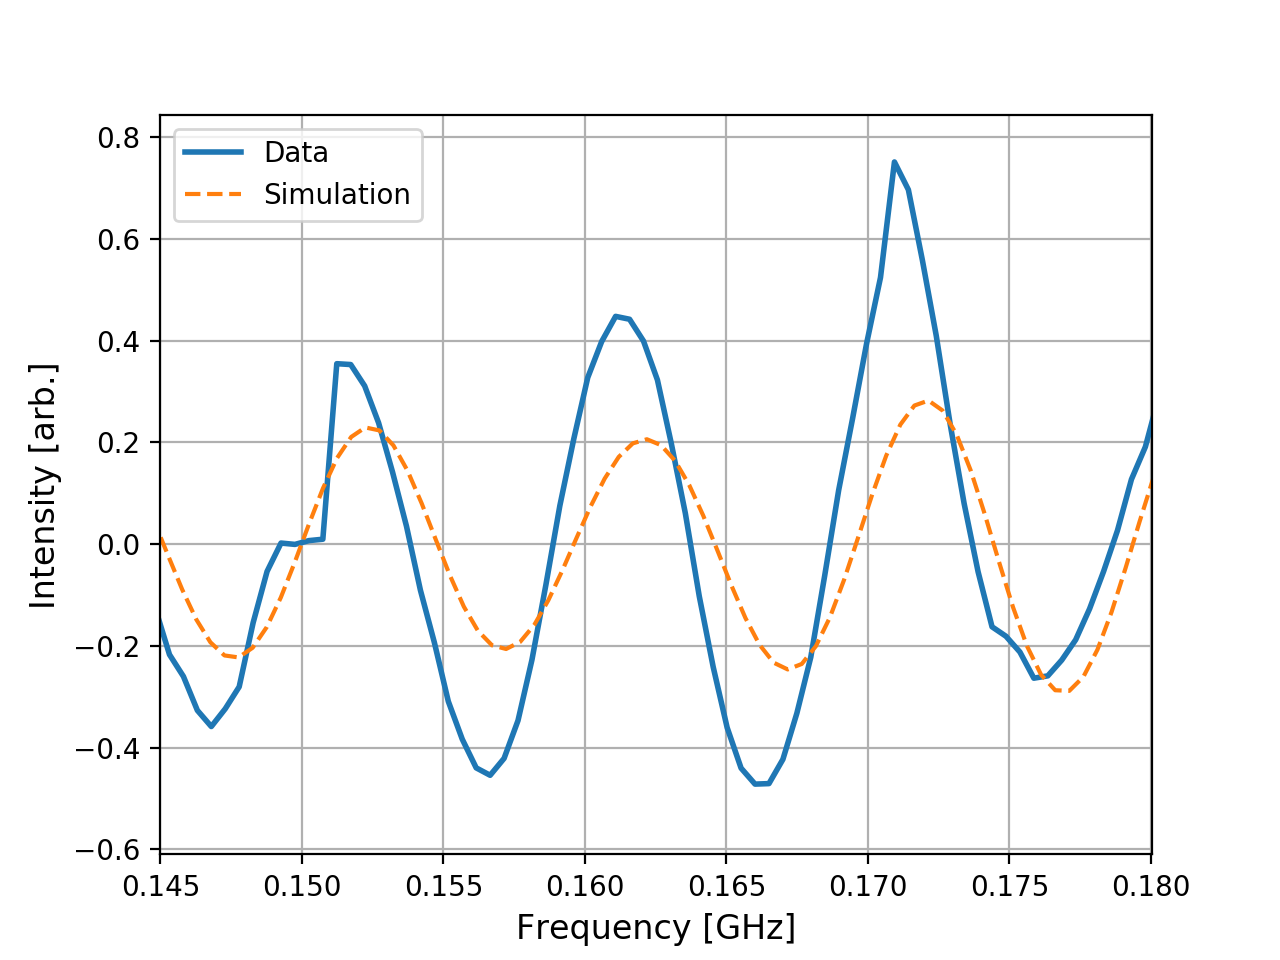
\includegraphics[width=0.7\textwidth]{chapters/global_signal/figures/data_sim_freq.png}
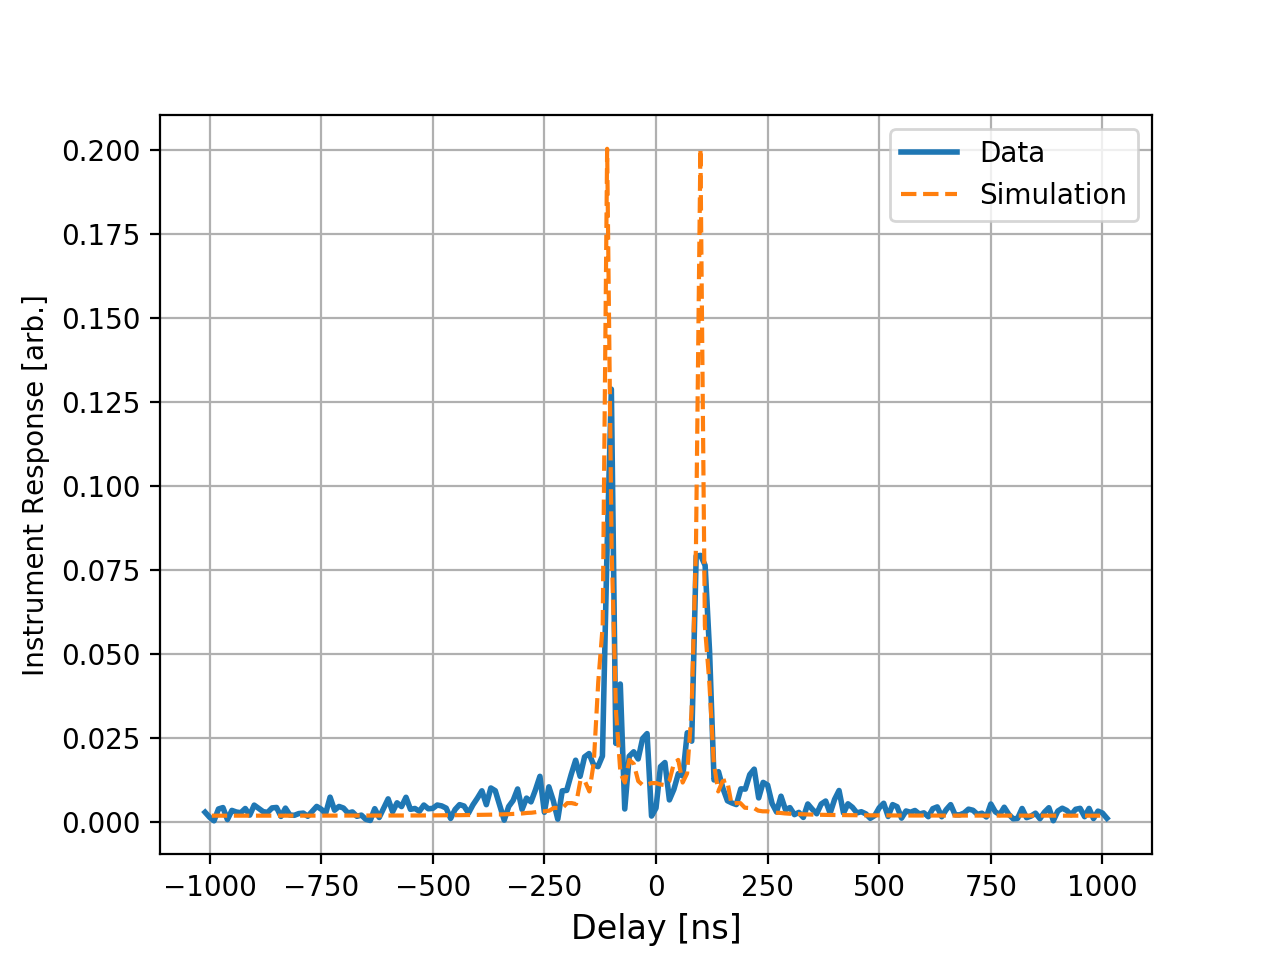
\includegraphics[width=0.7\textwidth]{chapters/global_signal/figures/data_sim_delay.png}
\caption[Comparison of time-averaged PAPER-128 visibilities to the simulated transfer function. ]{Comparison of time-averaged, LST-binned PAPER-128 visibilities to the simulated transfer function in the `nn' polarization. Upper and lower panels show the spectra in frequency and delay space. See the text for discussion.}
\label{fig:global_signal_data_vs_sim}
\end{figure}

The imperfect alignment of the oscillatory spectra may have been due to some frequency-dependent phase slope, possibly from an imperfect projection of redundant calibration degeneracies \citep[e.g.][Chapter~\ref{chapter:polcal}]{Dillon.17}. A more likely source of the misalignment was imperfect modelling of the beam. Higher $\ell$ values introduce additional spherical Bessel functions, each with their own phase that will superimpose for the final value of $\Xi(\hat{b},\nu)$.
\cite{Presley.15} provided an optimal quadratic estimator formalism to address this problem, which may be a promising route to pursue in future investigations.

The amplitude of the observed spectrum in frequency space increased towards higher frequencies, the opposite direction as predicted by the simulations and as expected for a signal tied to low-frequency synchrotron radiation \citep{Mozden.17}. The cause of this effect was unclear, but may be due to imperfect wide-band bandpass calibration\footnote{Note that such imperfections were unlikely to affect the power spectra reported in Chapter~\ref{chapter:eor_window_psa128}, as these used only a narrow range of frequencies.}.

\section{Discussion}

This analysis was an exploratory one, driven by investigations in to time-averages from PAPER-64 data as reported in the public HERA memo \#6. In that memo I investigated the impact of calibration errors and antenna cross-talk on time-averaged visibilities, showing that D-term leakage (e.g. Chapter~\ref{chapter:polcal}) could introduce low levels of spectral structure into the time-average, broadening the `wings' of horizon-power in delay space. Understanding the cause and shape of this delay space power is essential for obtaining EoR power spectra at $k$-values close to the foreground wedge.

The above analyses have shown that the PAPER beam and sky signal are quite accurately described by a low number of spherical harmonic modes. In our toy model we obtained delay-space signatures similar to those observed in data using only the ($\ell,m$)=(0,0) mode of the beam and sky, which had a relatively simple analytical form. The selection rules in our formalism do allow an arbitrary number of even $\ell$ modes to contribute to $\Xi(\hat{b},\nu)$, and developing a better understanding of those contributions may lead to a resolution to some of the problems described in the previous Section. Furthermore, a more advanced understanding of the effect of mis-calibration on the data that exceeds the conjectures above may resolve the offset between data and simulation. There may also be redundant calibration schemes that could provide an estimate of $\Xi(\hat{b},\nu)$ directly from the observed data.

HERA \citep{deBoer.17} will represent the most powerful low-frequency interferometer of its kind, with far more redundant baselines to average-over and experiment with in its search for the EoR power spectrum. However, it may not be the best instrument for a search for the global signal. Its faceted dish structure leads to smaller beams, which in turn leads to a large number of spherical harmonic modes required for its description. This complicates an accurate simulation of $\Xi(\hat{b},\nu)$ and hence the extraction of the global signal from observations. Interferometers specifically designed to target the global signal and adhere to prescriptions set by \cite{Venumadhav.16} may be more fruitful efforts.

We have shown that the global signal is, in theory, detectable by an interferometer. Our exploration with PAPER-128 data yielded imperfect but promising results. We detected a time-constant signal that is characterized by the length of the baseline used for the measurement; it was not simply electrical crosstalk. We may be quite close to a characterization of monopole power, following a relatively simple scheme. Much more work is required before a definitive claim of a detection, but in the meantime, our present observations remain exciting.

\section*{Note: interpretation in light of \cite{Venumadhav.16}}
The paper by \citealt{Venumadhav.16} conceptualizes a single
interferometer receiving element as a lossless electromagnetic junction, and as
such obeys conservation of energy on a microscopic level. As a consequence, the
entire array can be treated as being unitary, with input and output
corresponding to the sky, readout channels, and dissipative elements. By
invoking unitarity, the authors of \citealt{Venumadhav.16} show that a general interferometer is
only sensitive to the monopole moment either through cross-talk between
elements, or through coupling of distinct elements to a common dissipative noise
source. Explicitly, Equation~21 of \citealt{Venumadhav.16} can be written as:
\begin{equation}
\frac{1}{k_\mathrm{B}} \frac{\partial}{\partial\bar{T}_s} \left\langle\psi_{c_i}^* \psi_{c_j}\right\rangle =
- \sum_k U(c_i; c_k)^* U(c_j; c_k) - \sum_{d_k} \frac{1}{k_\mathrm{B}} \frac{\partial}{\partial T_{d_k}} \left\langle\psi_{c_i}^* \psi_{c_j}\right\rangle, 
\label{eqn:21V16}
\end{equation}
where ${\bar{T}_s}$ is the monopole moment (position-independent portion) of the
sky signal, $\psi_i$ is the amplitude of the electromagnetic vector potential
$\vec{A}$ for a given frequency and polarization in a particular readout channel
$i$, $U(c_i; c_j)$ is the cross-talk between readout channels $i$ and $j$, $d_k$
is the set of dissipative elements of the interferometer, $T_{d_k}$ is the
effective noise temperature of dissipative element $d_k$, and $k_\mathrm{B}$ is
Boltzmann's constant. Accordingly, one consequence of \citealt{Venumadhav.16} is that a ``perfect''
interferometer (one with no cross-talk or losses) is insensitive to the monopole
moment. Mathematically, the no cross-talk condition equates to the elements
$U(c_i; c_j) = 0$ for all $i \neq j$, and the lossless condition means that
$U(c_i; d_k) = 0$ for all readout channels $i$ and dissipate elements $k$.

In the main body of this Chapter, we showed that when directly computing the
integral of the interferometer equation, there is indeed sensitivity to the
global signal if the individual elements have certain properties (see
Section~\ref{sec:global_signal_math} for these requirements listed explicitly). In the
language of \citealt{Venumadhav.16}, we have assumed that there is indeed cross-talk between
individual receiving elements. Specifically, since most of the sensitivity to
the sky monopole comes from the baseline connecting two antennas, both antennas
must be sensitive to signal along the line-of-sight to the horizon. Because the
antenna closer to the horizon is not electromagnetically transparent to the
incoming radiation -- indeed, there would be no detection of the signal if it
were -- it must necessarily re-broadcast the incoming radiation. This radiation
is then detected by the antenna farther from the horizon, which leads to
over-the-air cross-talk between the two antennas. Thus, in the language of \citealt{Venumadhav.16},
the matrix element $U(c_i; c_j)$ is non-zero for this pair of antennas $i$ and
$j$, and as such there is sensitivity to the global signal. If we assume the
interferometer is lossless (but \textit{not} that there is no cross-talk), then
the sensitivity to the global signal can be expressed as:
\begin{equation}
\frac{1}{k_\mathrm{B}} \frac{\partial}{\partial\bar{T}_s} \left\langle\psi_{c_i}^* \psi_{c_j}\right\rangle =
- \sum_k U(c_i; c_k)^* U(c_j; c_k). 
\label{eqn:losslessTs}
\end{equation}
We note that in \citealt{Venumadhav.16}, for the lossless case, the unitarity constraint of the
system can be expressed as:
\begin{equation}
\sum_{\alpha,a} U(c_i; \alpha, \hat{n}_a)^* U(c_j; \alpha, \hat{n}_a) + \sum_k U(c_i; c_k)^* U(c_j; c_k) = 0,
\end{equation}
where $U(c_i; \beta, \hat{n}_b)$ is the amount of signal captured in readout
channel $c_i$ of polarization $\beta$ and pixel $\hat{n}_b$ of the sky (once it
has been discretized, see Appendix~A of \citealt{Venumadhav.16}). This also assumes the readout
channels are distinct, \textit{i.e.}, $i \neq j$. This relation can be
substituted into Equation~\ref{eqn:losslessTs}, which leads to:
\begin{equation}
\frac{1}{k_\mathrm{B}} \frac{\partial}{\partial\bar{T}_s} \left\langle\psi_{c_i}^* \psi_{c_j}\right\rangle =
\sum_{\alpha, a} U(c_i; \alpha, \hat{n}_a)^* U(c_j; \alpha, \hat{n}_a).
\label{eqn:skyTs}
\end{equation}
Further, in the limit of a lossless interferometer, the formalism of \citealt{Venumadhav.16} leads
to the traditional interferometer equation. Specifically, for two antennas $c_1$
and $c_2$ at a frequency $\nu_m$, the interferometer equation can be expressed as:
\begin{equation}
\sum_{\alpha, a} U(\nu_m, c_1; \alpha, \hat{n}_a)^* U(\nu_m, c_2; \alpha, \hat{n}_a) k_\mathrm{B} T_s(\hat{n}_a) =
\int {\rm d}\hat{n} A(\nu_m, \hat{n}) \frac{\nu_m^2}{c^2} k_\mathrm{B} T_s (\hat{n}_a) e^{2\pi i \nu_m (\vec{r}_2 - \vec{r}_1) \cdot \hat{n}_a},
\end{equation}
which is simply the visibility equation, where the sky signal has been converted to a brightness temperature.